\documentclass[../sk-egzamin.tex]{subfiles}

\begin{document}

\question{
Proszę opisać protokół IPSec.
}

\subsection*{IPSec}
\begin{itemize}
    \item Działa w \textbf{warstwie sieci} \parit{trzeciej}.

    \item \textbf{Bardziej framework wykorzystujący inne protokoły.}

    \item Pewne \textbf{uzupełnienie IPv4, włączone do IPv6}.

    \item Wykorzystywany do szyfrowania i sprawdzania autentyczności i
    integralności przesyłanych danych z dowolnej aplikacji.

    \item Proces szyfrowania i deszyfrowania jest \textbf{niewidoczny}
    dla użytkownika.

    \item Głownymi częściami IPSec są \textbf{protokoły}:
    \begin{itemize}
        \item \textbf{Authentication Headers} \parit{AH}.
        \begin{itemize}
            \item \textbf{Nie ma szyfrowania - wykorzystywany HMAC}.
            \item Umożliwia sprawdzenie autentyczności komputerów
            uczestniczących w transmisji.
            \item Sprawdzenie integralności danych.
            \item Nagłowek IP oraz dane są zabezpieczone przed modyfikacją.
        \end{itemize}
        \item \textbf{Encapsulating Security Payloads} \parit{ESP}.
        \begin{itemize}
            \item Zapewnia \textbf{szyfrowanie}, autentyczność i integralność
            danych.
            \item Samodzielnie lub z AH, na ogół sam ESP jest wykorzystywany.
        \end{itemize}
    \end{itemize}
\end{itemize}

Przed przesyłaniem danych strony komunikujące się uzgadniają szczegóły takie
jak sposób uwierzytelniania, wymiana kluczy, algorytmy szyfrowania.

\subsection*{Polityki stosowania IPSec}
Można ustalić zasadę kiedy IPSec ma być automatycznie zastosowany.

\begin{itemize}
    \item \textbf{Client} \parit{respond only} - transmisje bez IPSec,
    chyba że druga strona zażąda IPSec.
    \item \textbf{Server} \parit{request security} - żądanie transmisji IPSec,
    ale jeśli druga strona nie implementuje IPSec, to komunikacja bez.
    \item \textbf{Secure server} \parit{require security} - żądanie transmisji
    IPSec, jeśli druga strona nie implementuje IPSec, to komunikacja nie jest
    kontynuowana.
\end{itemize}


\subsection*{Tryby działania IPSec \parit{zarówno AH jak i ESP}}
\begin{itemize}
    \item \textbf{Transportu} \parit{w sieci lokalnej}
    między dwoma punktami końcowymi transmisji.
    \begin{itemize}
        \item Prostszy,
        wymaga mniej przetwarzania danych, ale \textbf{mniej użyteczny}.
        \item Nagłówek AH jest wstawiany \textbf{między} nagłowek IP i TCP.
    \end{itemize}
    \item \textbf{Tunelowania} -
    szyfrowanie w niezabezpieczonej części sieci (np. dane między
    biurami przesyłane przez Internet).
    \begin{itemize}
        \item Więcej pracy, ale \textbf{bardziej użyteczny}.
        \item Pakiet IP w pakiecie IP.
    \end{itemize}

    \textbf{IPSec (ESP w trybie tunelowym) może być wykorzystany do realizacji
    VPN – Virtual Private Network}.
\end{itemize}

\subsection*{Metody uwierzytelniania w IPSec}
\begin{itemize}
    \item \textbf{Kerberos}
    \item \textbf{Oparty o certyfikaty cyfrowe}
    \item \textbf{Klucz dzielony} - przechowywany we właściwościach napis
    jednakowy dla obu komunikujących się stron.
\end{itemize}

\subsection*{Filtry IPSec}

Filtr IPSec pozwala na automatyczne przepuszczenie datagramów IP, blokowanie
lub użycie negocjacji (i w konsekwencji użycie IPSec) w zależności od źródła i
miejsca docelowego IP, protokołu transportowego, portów źródłowych i docelowych.

\subsection*{Obrazki}

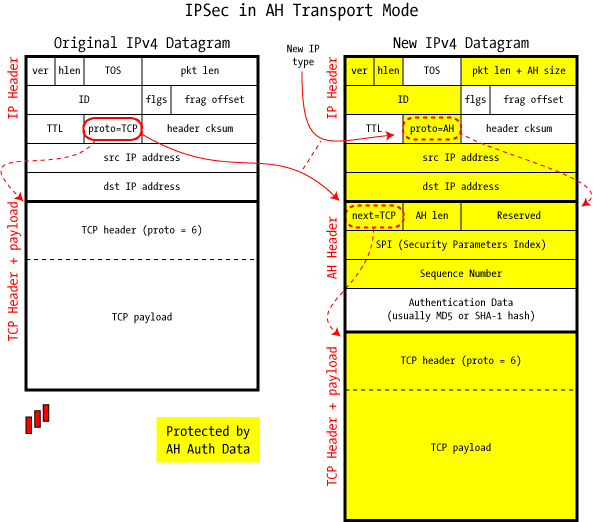
\includegraphics[width=\textwidth]{ipsec-ah-transport}

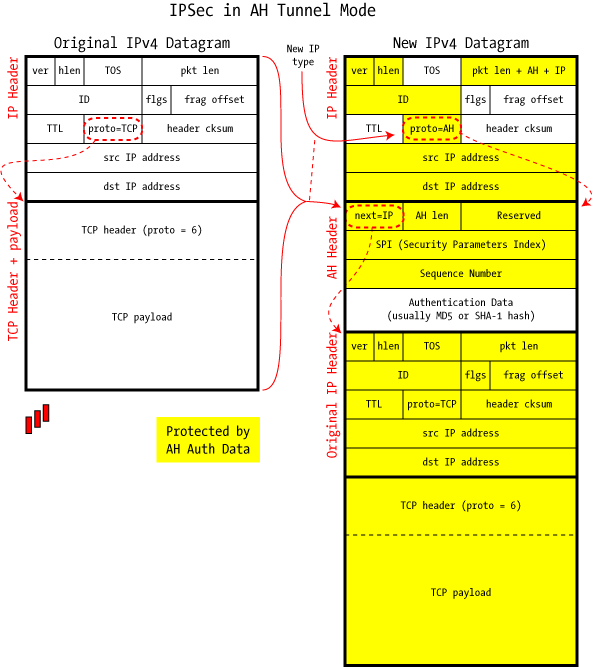
\includegraphics[width=\textwidth]{ipsec-ah-tunnel}

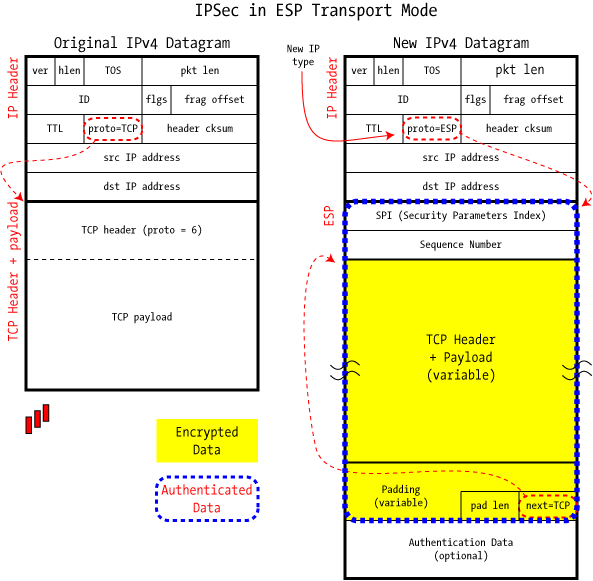
\includegraphics[width=\textwidth]{ipsec-esp-transport}

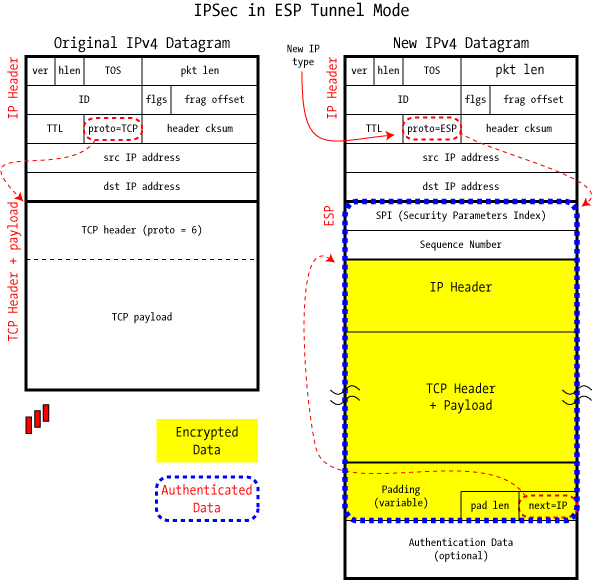
\includegraphics[width=\textwidth]{ipsec-esp-tunnel}

\pagebreak
\end{document}
